\documentclass[12pt,
border=1pt]{standalone}
\usepackage{pgfplots}
\usepackage{amsmath}
\usepackage{amssymb}

\pgfplotsset{compat=newest,
	width=6cm, height=5cm,
	xtick pos=left, ytick pos=left,
	%            scaled x ticks=real:1e-6,
}
% Kernel 2 FP64
\begin{document}
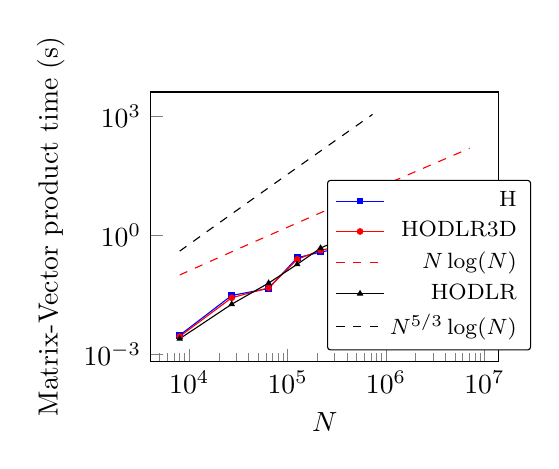
\begin{tikzpicture}[every mark/.append style={mark size=1pt}]
	\begin{axis}[xlabel={$N$},
	ylabel={Matrix-Vector product time (s)},
%		legend pos=south east,
		legend style={
                at={(0.8,0.04)},
               anchor=south,
               legend columns=1,
               cells={anchor=east},
              font=\footnotesize,
               rounded corners=1pt,
               },
		xmode = log,
	    ymode = log,
	   % xmin = 1e3,
	   % xmax = 1e6,
	   % ymin = 1e-10,
	   % ymax = 1e-0,
	   % xtick={1e-10, 1e-8, 1e-6,  1e-4,  1e-2},
	   % ytick={1e-8, 1e-6,  1e-4,  1e-2, 1e-0}
		]
		
		\addplot[
		color=blue,
		mark=square*,
		] coordinates {
(8000,0.002999)
(27000,0.030109)
(64000,0.045156)
(125000,0.267557)
(216000,0.372911)
(343000,0.465301)
(512000,0.677534)
(729000,0.997064)
(1000000,2.974710)
(1331000,4.362850)
(1728000,4.052130)
(2197000,4.732000)
(2744000,5.841680)
(3375000,7.356550)
(4096000,6.929720)
(4913000,8.587820)
(5832000,12.358000)
(6859000,11.149200)
		};
		\addplot[
		color=red,
		mark=*,
		] coordinates {
(8000,0.002788)
(27000,0.026326)
(64000,0.046711)
(125000,0.244085)
(216000,0.414865)
(343000,0.522523)
(512000,0.652037)
(729000,0.870077)
(1000000,2.607710)
(1331000,3.121390)
(1728000,3.839270)
(2197000,4.662530)
(2744000,5.792950)
(3375000,6.832690)
(4096000,8.439400)
(4913000,9.605090)
(5832000,12.032300)
(6859000,13.236200)
% (7077888,11.328600)
		};
		\addplot[mark=none, red, dashed][
		domain = 8000:7077888,
		] {(pow(10,-5.5)*x*log10(x)};
\addplot[
		color=black,
		mark=triangle*,
		] coordinates {
(8000,0.002446)
(27000,0.018124)
(64000,0.061574)
(125000,0.183393)
(216000,0.469178)
(343000,0.788424)
(512000,1.657480)
(729000,4.099990)
		};
\addplot[mark=none, black, dashed][
		domain = 8000:729000,
		] {(pow(10,-7.5)*pow(x,5/3)*log10(x)};
		\legend{H, HODLR3D, $N\log(N)$, HODLR, $N^{5/3}\log(N)$}
		\end{axis}
\end{tikzpicture}
\end{document}